\chapter{Asking Millionaires How They Got Rich in Dallas}

This chapter comes from a School of Hard Knocks field lecture rather than a blackboard performance, but we should not mistake the absence of chalk for the absence of structure. As we move through Dallas, the same few variables keep returning under different names: cash in and cash out, the capital buffer that protects a growing firm, the difference between salary and ownership, the governance problem inside financing, and the option value of cash when the environment turns hostile. No validated mathematical screenshots remain for this lecture, so every displayed formula below is a careful reconstruction from the spoken argument.

\section{Dallas as a Field of Inquiry}

The episode begins with a teaser reel: large revenue numbers, statements of coming from nothing, and the visible symbol of the Rolls Royce. Then the host resets the scene and states the program more plainly. Dallas is one of the richest cities in the world, and the plan is to move through it, find wealthy operators, and ask how they got there.

That opening matters because the lecture does not begin by explaining a doctrine. It begins by creating a search. We are shown repeated refusals, interruptions, and half-answers before we are given a real conversation. The effect is to make each successful interview feel earned. These are not studio monologues delivered on cue; they are fragments won out of a noisy city.

There is also a recurrent threshold question: ``Have you ever been broke before?'' This is a good opening move. Before we trust advice, we are asked to locate the speaker inside financial history. Success is not heard in abstraction; it is heard against struggle, or against the absence of struggle.

\begin{definition}
In these notes each interview is treated as a three-part object:
\begin{itemize}
\item an anecdote, which tells us who is speaking;
\item a claim, which tells us what the speaker asserts;
\item a mechanism, which is the part we may formalize and carry forward.
\end{itemize}
\end{definition}

With that method in hand, we can follow the lecture as it unfolds. The city gives us one case, then another, and the host keeps doing the same thing a good lecturer does: he asks the next question exactly where the previous answer leaves an opening.

\section{Banking: Acquisition, Focus, and the Cost of Growth}

The first long case arrives after the refusal sequence. The interviewee says he runs banks and that his businesses today make roughly \(500\) million a year. Once that scale is on the table, the lecture turns quickly from biography to mechanism: how does one scale to nine figures?

The answer is terse and operational. The business grew mostly through acquisition, and in banking, as he puts it, the game is to buy them and strip out costs. If we preserve only the mathematical skeleton of that statement, we get
\begin{equation}
\Pi_{\mathrm{post}} \approx \Pi_{\mathrm{legacy}} + \Pi_{\mathrm{target}} + \Delta \Pi_{\mathrm{cuts}}.
\end{equation}
This is not a merger model in any full corporate-finance sense. It is simply the cleanest transcript-backed way to write what the interviewee says he did: add targets, then improve economics by removing cost.

The next move in the lecture is focus. The banker says he has stayed in banking for \(44\) years and argues that ``plan B'' is the enemy of ``plan A.'' We should be careful here. This is not a theorem about decision theory. But the local mechanism is still intelligible: concentration preserves effort, while fallback plans can leak effort away from the main line of attack.

The host then sharpens the conversation by asking what keeps businesses from making it past five years. He cites a very high failure rate and asks for the common mistake. That is the moment at which the lecture's first genuine invariant appears.

\subsection{Question \& Answer}

\paragraph{Question.} Why do firms that appear to be growing still fail?

\paragraph{Answer.} Because growth in revenue is not the same thing as growth in survivable cash.

The interviewee says that many businesses grow fast, imagine themselves to be healthy, and then outstrip their capital. We can write the relevant bookkeeping in a compact form. Let
\begin{equation}
CF_t = \mathrm{In}_t - \mathrm{Out}_t
\end{equation}
denote net cash flow during period \(t\), and let \(K_t\) denote the liquid capital buffer available at the start of that period. Then the simplest update rule is
\begin{equation}
K_{t+1} = K_t + CF_t.
\end{equation}
Iterating over \(n\) periods gives
\begin{equation}
K_{t+n} = K_t + \sum_{j=0}^{n-1} CF_{t+j}.
\end{equation}

\begin{proposition}
If a firm expands in such a way that \(CF_{t+j}<0\) for \(j=0,\dots,n-1\), then the capital buffer shrinks:
\begin{equation}
K_{t+n} < K_t.
\end{equation}
\end{proposition}

\begin{proof}
From the update rule,
\[
K_{t+n} = K_t + \sum_{j=0}^{n-1} CF_{t+j}.
\]
If each term in the sum is negative, then the sum is negative. Hence \(K_{t+n}<K_t\).
\end{proof}

The algebra is elementary, but that is exactly why it is useful. A business may be expanding headcount, inventory, integration costs, or working capital demands faster than it is building liquid resilience. In that situation, the thing called ``growth'' is also the thing that is eating the life of the firm.

The host does the right thing after this exchange: he stops and recaps. He does not summarize the interview as ``a man who made a lot of money in banking.'' He summarizes it as ``cash flow is king.'' That recap matters because it converts an interview into a portable rule, and once that rule exists the next cases can be heard against it.

\section{Capital Structure, Negotiation, and Control}

Once we have seen that growth can destroy a business by starving its capital buffer, the next question becomes unavoidable: how should that growth be financed? The banker answers in one word: equity.

But the answer is not simply ``get investors.'' The host immediately pushes on the danger built into that advice, and the interviewee responds with a control warning: do not let any one investor become too large, or you will end up working for him.

Let \(\alpha_{\max}\) denote the largest outside investor share, and let \(C_{\mathrm{founder}}\) denote effective founder control. Then the interviewee's warning can be written schematically as
\begin{equation}
\alpha_{\max} \uparrow \quad \Longrightarrow \quad C_{\mathrm{founder}} \downarrow.
\end{equation}
No numerical threshold is given in the lecture, and we should not invent one. The point is structural. Financing changes two things at once:
\begin{itemize}
\item it changes the cash available to the enterprise,
\item it changes the command structure of the enterprise.
\end{itemize}

This is why the transcript does not flatten into simple pro-equity rhetoric. What matters is not just whether capital enters, but also on what terms it enters.

The same interview then folds outward into a more general claim about entrepreneurship. Not everyone is built for it, the banker says, but if one wants to make real money, one usually ends up having to make it work for oneself. That sentence is placed carefully in the transcript. It comes after the discussion of control, as if to say that the upside of entrepreneurship cannot be separated from the burden of carrying command.

The host then asks for negotiation advice, and the banker answers with a compact rule: walk away. His best deals, he says, were the ones he walked away from and that later came back. In the notes we can record the principle in a reservation-value form:
\begin{equation}
V_{\mathrm{deal}} < V_{\mathrm{walk}} \quad \Longrightarrow \quad \text{walk away}.
\end{equation}
Again, this is a reconstruction, not a spoken formula. But it fits the lecture's logic exactly. The option not to transact is part of bargaining power. This will matter again at the end of the chapter, when cash reserves create the option not to buy until other people are forced to sell.

\section{Consulting, Equity, and Family Trajectory}

After the host's cash-flow recap, the lecture turns to a retired consultant and former business owner whose clients included large firms such as Frito-Lay, American Airlines, and TXU Energy. The first thing to notice is that the cash-flow warning appears again. A different speaker, a different industry, and yet the same diagnosis returns: many businesses have a good product or service but do not know how to manage cash flow.

That repetition is important. We are no longer dealing with a one-off opinion. The lecture is beginning to show us a pattern across sectors.

But this second case adds something the first one did not. The consultant reports that his highest annual personal income was between \(8\) and \(10\) million, and when the host asks how that jump happened, the answer is unmistakable: equity ownership. Salary and bonus existed, but the large step up came through dividends.

The clean way to write the structure is
\begin{align}
Y &= S + B + D,\\
D &= q\,\Pi_{\mathrm{dist}},
\end{align}
where \(Y\) is total personal yearly income, \(S\) is salary, \(B\) is bonus, \(D\) is dividends, \(q\) is the effective ownership share, and \(\Pi_{\mathrm{dist}}\) is the distributable profit pool. The lecture's conceptual split is then
\begin{equation}
Y_{\mathrm{labor}} = S+B,
\qquad
Y_{\mathrm{ownership}} = D.
\end{equation}

\subsection{Question \& Answer}

\paragraph{Question.} How does a high earner cross from seven figures of compensation into eight figures of wealth?

\paragraph{Answer.} By moving from labor-linked income into ownership-linked income.

The transcript is approximate, but it is numerically suggestive enough to build a simple example. If the consultant's total yearly income \(Y\) is between \(8\) and \(10\) million, and if salary plus bonus is only about \(750{,}000\), then most of the total must be carried by dividends:
\begin{equation}
D \approx Y-(S+B).
\end{equation}
In words, the dividend component must then account for something like \(7.25\) to \(9.25\) million of the total. The exact number is less important than the category change. The lecture is teaching us that very large personal income is not simply more salary; it is often a claim on the firm's profit stream.

The host then asks what skill was hardest to master, and the answer is not a technical skill in consulting. It is leadership: casting a vision for a small team so that it can become a large one. That is a subtle but important turn in the lecture. We have moved from bookkeeping to social organization. Wealth at this scale requires not only a balance sheet but a future that other people are willing to inhabit.

\begin{figure}[h]
\centering
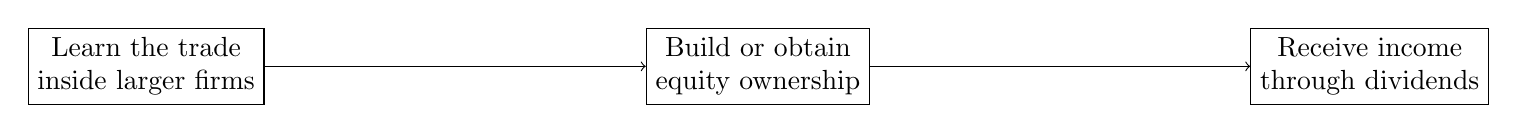
\begin{tikzpicture}[x=3.7cm,y=1.7cm]
\node[draw, rectangle, align=center] (a) at (0,0) {Learn the trade\\inside larger firms};
\node[draw, rectangle, align=center] (b) at (2.1,0) {Build or obtain\\equity ownership};
\node[draw, rectangle, align=center] (c) at (4.2,0) {Receive income\\through dividends};
\draw[->] (a) -- (b);
\draw[->] (b) -- (c);
\end{tikzpicture}
\caption{A transcript-derived social-mobility sequence: apprenticeship produces competence, competence makes ownership possible, and ownership opens the profit channel that salary alone does not provide.}
\end{figure}

This figure is justified by the narrative that follows. The consultant says he came from nothing, learned his trade during roughly ten years inside big firms, and then spent the next twenty to twenty-five years building companies of his own. The host then asks how he changed his family's trajectory, and the answer is almost diagrammatic: first learn the trade while working for the big man, then step out and build.

Two more remarks complete the rhythm of this case. First, the consultant says, ``Love what you do and you'll never work a day in your life.'' That sentence belongs here because it is placed between the income discussion and the family-trajectory discussion. It serves as the human motive that links technique to endurance. Second, when asked for the greatest lesson of entrepreneurship, he answers with the burn-the-ships mentality. Most fail, so retreat cannot be the default setting. That is not formal mathematics, but it is the motivational edge that the lecture uses to keep ownership from sounding like passive entitlement.

\section{Restaurants, Risk, Support, and Land}

The next case changes the balance of the lecture. We move from banking and consulting into restaurants, and the tone shifts from the power of ownership to the burden of it. The interviewee says he owned restaurants for ``too damn long,'' bought a franchise so somebody else would do the heavy thinking, and also ran TGI Fridays. He reports business scale of about a billion dollars across his career. Yet the lesson the host extracts is not one of glamour. It is one of organizational realism.

Asked where people go wrong, the answer is that they do not build a team that supports them, and they imagine themselves to be king. This is one of the sharpest leadership statements in the lecture. Firms fail not only because the numbers break, but because the leader imagines the firm to be a one-man projection rather than a structure supported by other capable people.

\subsection{Question \& Answer}

\paragraph{Question.} Is it always better to own the business yourself?

\paragraph{Answer.} No. Ownership raises upside, but it also raises downside exposure.

The restaurant executive says this more bluntly than anyone else in the lecture. If you own the business, you may have to put up your house and your assets. If you work for the other guy, the downside is smaller: lose the job, then get another one.

Let \(L(\mathcal{O})\) denote downside exposure in the owner state and \(L(\mathcal{E})\) downside exposure in the employee state. The lecture supports the qualitative comparison
\begin{equation}
L(\mathcal{O}) > L(\mathcal{E}).
\end{equation}
This is not a universal career theorem. It is the speaker's way of naming how ownership concentrates risk. The chapter needs that sentence because it pushes back against a too-easy reading of the previous sections. Equity is powerful, but equity also exposes.

The interview then moves outward again, this time from the firm to the household. The host asks how important it is to choose the right life partner, and the executive says support at home is essential. If the home front is miserable, work life and health collapse with it. Here the lecture quietly widens the system boundary once more. We are not only analyzing enterprises. We are analyzing the conditions under which a human being remains functional enough to run one.

When asked how to become a millionaire in \(2024\), the same interviewee says he goes long on real estate and adds that ``real estate never goes down.'' We should preserve the force of the statement while keeping the logical temperature under control.

\begin{remark}
The phrase ``real estate never goes down'' should be read as an interview claim, not as a market theorem. The more careful argument comes in the follow-up: the people who really made money owned the land and the properties rather than merely leasing or renting them.
\end{remark}

That is a much stronger sentence. It changes the claim from a naïve monotonicity statement into a more coherent ownership statement: the deeper asset is the property itself, especially when held for a long horizon.

At this point the lecture briefly interrupts itself for a School of Mentors announcement. The interruption is real, and it should be acknowledged. But analytically it functions only as a pause. When the interviews resume, they return to the same structure, now with a more explicit emphasis on ruin, rebuilding, and cash reserves.

\section{Recovery, Self-Investment, and Cash Optionality}

The final major case begins where the opening teaser began: with the Rolls Royce. The speaker is an entrepreneur, a former Marine, and a business owner for \(25\) years, with top-line revenue of roughly \(40\) million. But once again the visible object is only bait. The lecture quickly moves toward mechanism.

The first mechanism is self-investment. The speaker says that when he asked a Goldman Sachs man how quickly \(10\) million could become \(20\) million, the answer was: stop thinking of the next doubling as something external. Invest back into yourself and into your own business. Asked what that means, he names the components: skills, associations, relationships, reputation. The lecture is thus closing a loop that began earlier. Capital is not only money held outside the self; it is also the enlargement of one's own capacity to produce, attract, and negotiate.

The second mechanism is recovery after ruin. The speaker says he first became a millionaire in his thirties, lost it in a bad relationship, and rebuilt in his forties. The host then asks how one bounces back. The answer comes in two registers at once. One is spiritual: the worst position is the best position, because that is when God gets heard. The other is practical: the bottom strips away illusion and makes one remember the source of one's resources. Whether or not we adopt the theological language, we should preserve the structural point. The lecture treats collapse not only as a subtraction of wealth but as a re-ordering of attention.

The third mechanism is epistemic. Asked what billionaires do differently, the speaker says they ask more questions and enter rooms not assuming they already know everything. This is one of the most elegant moments in the episode because it folds the method of the interviewer back into the content of the interview. Curiosity is no longer just a filming device; it becomes part of the subject matter.

\subsection{Question \& Answer}

\paragraph{Question.} How does a downturn become an opportunity rather than merely a catastrophe?

\paragraph{Answer.} By entering the downturn with liquid reserves while others enter it with forced-sale pressure.

The final advice about getting a Rolls Royce in \(2024\) is actually a local theory of optionality. When rates rise and people who did not save begin to strain, assets once sold at a premium begin to clear at a discount. Let \(P_{\mathrm{peak}}\) denote the earlier price and \(P_{\mathrm{distress}}\) the forced-sale price. The transcript supplies a discount band through examples of \(20\%\), \(30\%\), \(40\%\), even \(50\%\). So we may write
\begin{align}
P_{\mathrm{distress}} &= (1-\delta)P_{\mathrm{peak}},\\
0.2 \le \delta \le 0.5.
\end{align}

Let \(M_t\) denote reserves carried into period \(t\), and let \(s_t\) denote new saving during favorable conditions. The reserve dynamics are then
\begin{equation}
M_{t+1} = M_t + s_t.
\end{equation}
If \(Q_t\) denotes purchase optionality, the lecture's central implication is
\begin{equation}
M_t \uparrow \quad \Longrightarrow \quad Q_t \uparrow.
\end{equation}

\begin{figure}[h]
\centering
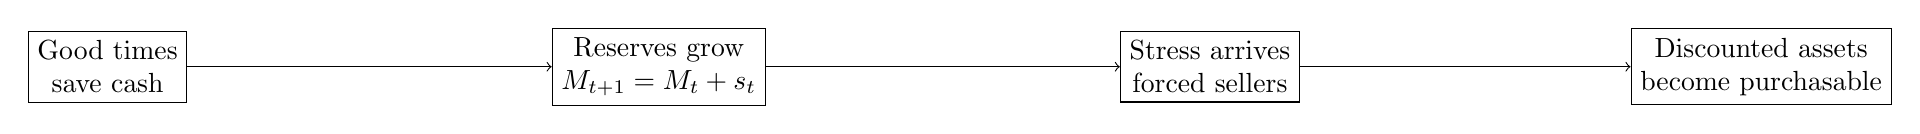
\begin{tikzpicture}[x=2.8cm,y=1.6cm]
\node[draw, rectangle, align=center] (a) at (0,0) {Good times\\save cash};
\node[draw, rectangle, align=center] (b) at (2.5,0) {Reserves grow\\\(M_{t+1}=M_t+s_t\)};
\node[draw, rectangle, align=center] (c) at (5.0,0) {Stress arrives\\forced sellers};
\node[draw, rectangle, align=center] (d) at (7.5,0) {Discounted assets\\become purchasable};
\draw[->] (a) -- (b);
\draw[->] (b) -- (c);
\draw[->] (c) -- (d);
\end{tikzpicture}
\caption{A transcript-derived optionality sequence: saving in good times does not look dramatic, but it is precisely what creates bargaining power when markets turn and others must sell.}
\end{figure}

\paragraph{Worked example.} Suppose a luxury vehicle carried a peak price
\[
P_{\mathrm{peak}} = 500{,}000,
\]
and suppose distress forces a \(30\%\) discount, so \(\delta=0.3\). Then
\begin{equation}
P_{\mathrm{distress}} = (1-0.3)\cdot 500{,}000 = 350{,}000.
\end{equation}
The object in the lecture happens to be a Rolls Royce, but the rule is larger than the car. Liquid cash acquires option value exactly when other people no longer have the luxury of waiting.

This ending is careful in its own way. The speaker does not say, ``Buy expensive things.'' He says: save in good times, because bad times make bargains visible only to those who arrive with liquidity. The lecture began with a flashy object, but it ends with a quiet principle of timing.

\section{Summary}

If we read the episode as a lecture rather than as a bag of clips, a coherent structure emerges. We begin with access and biography, then move into the first hard mechanism, which is cash flow. From there the lecture deepens into acquisition, control, and financing; then it shifts into the distinction between labor income and ownership income; then it widens again to leadership, household support, and risk concentration; and finally it closes with ruin, recovery, curiosity, and the option value of cash.

A compact summary of the chapter is this:
\begin{itemize}
\item revenue without liquid discipline is not durability;
\item equity changes the category of income, but it also changes the category of risk;
\item financing is never only about money, because it also redistributes control;
\item cash held in good times becomes bargaining power in bad times.
\end{itemize}

That is why the lecture feels richer than a collection of success stories. The city gives us anecdotes, but the host keeps pulling them toward mechanism. By the end, the central lesson is not merely that some people got rich. It is that wealth, on this telling, is built where operating skill, ownership, disciplined cash flow, and strategic patience meet.